\section{Evaluation}

Our evaluation seeks to answer the following questions:
\begin{enumerate}
    \item What is the abstraction overhead of eBQL? Do eBQL-generated queries have comparable
        performance to hand-optimized queries? (\S \ref{opt-eval})
    \item How do eBQL-generated queries compare to standard baseline eBPF programs? (\S
        \ref{baseline-eval})
    \item What is the actual overhead of the BPF subsystem, and what benefit does computation
        pushdown into the kernel have? (\S \ref{perf-drilldown})
\end{enumerate}

All evaluations run on a server machine with two Xeon Gold 6150 CPUs (36$\times $ 2.7 GHz) and 377
GiB of RAM. Persistent storage is provided by a Samsung 1TB NVM Drive. The systems runs Ubuntu 22.04
with Linux v5.15.

We evaluate eBQL and hand-written queries using a workload derived from real-world observability
use-cases. Specifically, a \textbf{RocksDB application} under high load continually executes
\texttt{get} commands, reading results from persistent storage. The RocksDB application runs $8$
writer threads concurrently, stopping once 50 million operations are completed.  RocksDB application
randomly selects from pre-generated set of $1,000,000$ keys, each containing a data value of 128
bytes, minimizing the effects of caching. A separate process attaches the eBPF program into the
kernel at the \texttt{sys\_enter\_pread64} tracepoint and collects and processes the outputted data.

Both applications are pinned to a fixed set of 12 CPUs using \texttt{taskset}, carefully chosen to
avoid interference from CPU hyperthreading (we briefly discuss the effect of restricting the number
of cores to 8, such that the RocksDB application then runs within a resource-constrained
environment, with worker threads having competing processes).

Before each benchmark, we run the RocksDB operation individually to reduce any disk caching effects.

\subsection{End-to-End Evaluation}
\label{opt-eval}

We first measure the performance of a query from an eBQL-generated eBPF program compared to a
hand-optimized eBPF program. Ideally, the abstraction overhead of eBQL's higher-level interface and
subsequent query processing steps should be minimal, and provide comparable performance to
hand-optimized programs with a fraction of the developer overhead.

We measure the read throughput achieved by RocksDB, first without any eBPF probes attached to
determine the baseline expected throughput, then with the eBQL-generated eBPF program and the
hand-optimized eBPF program. We also measure a wide range of read latency quantiles to evaluate if
either probe has a significant effect on tail latencies.

Figure \ref{fig:opt-eval-throughput} shows the RocksDB read throughput over the three measurements,
and figure \ref{fig:opt-eval-quantiles} shows the RocksDB read latencies across various quantiles.

\begin{figure}[htpb]
    \centering
    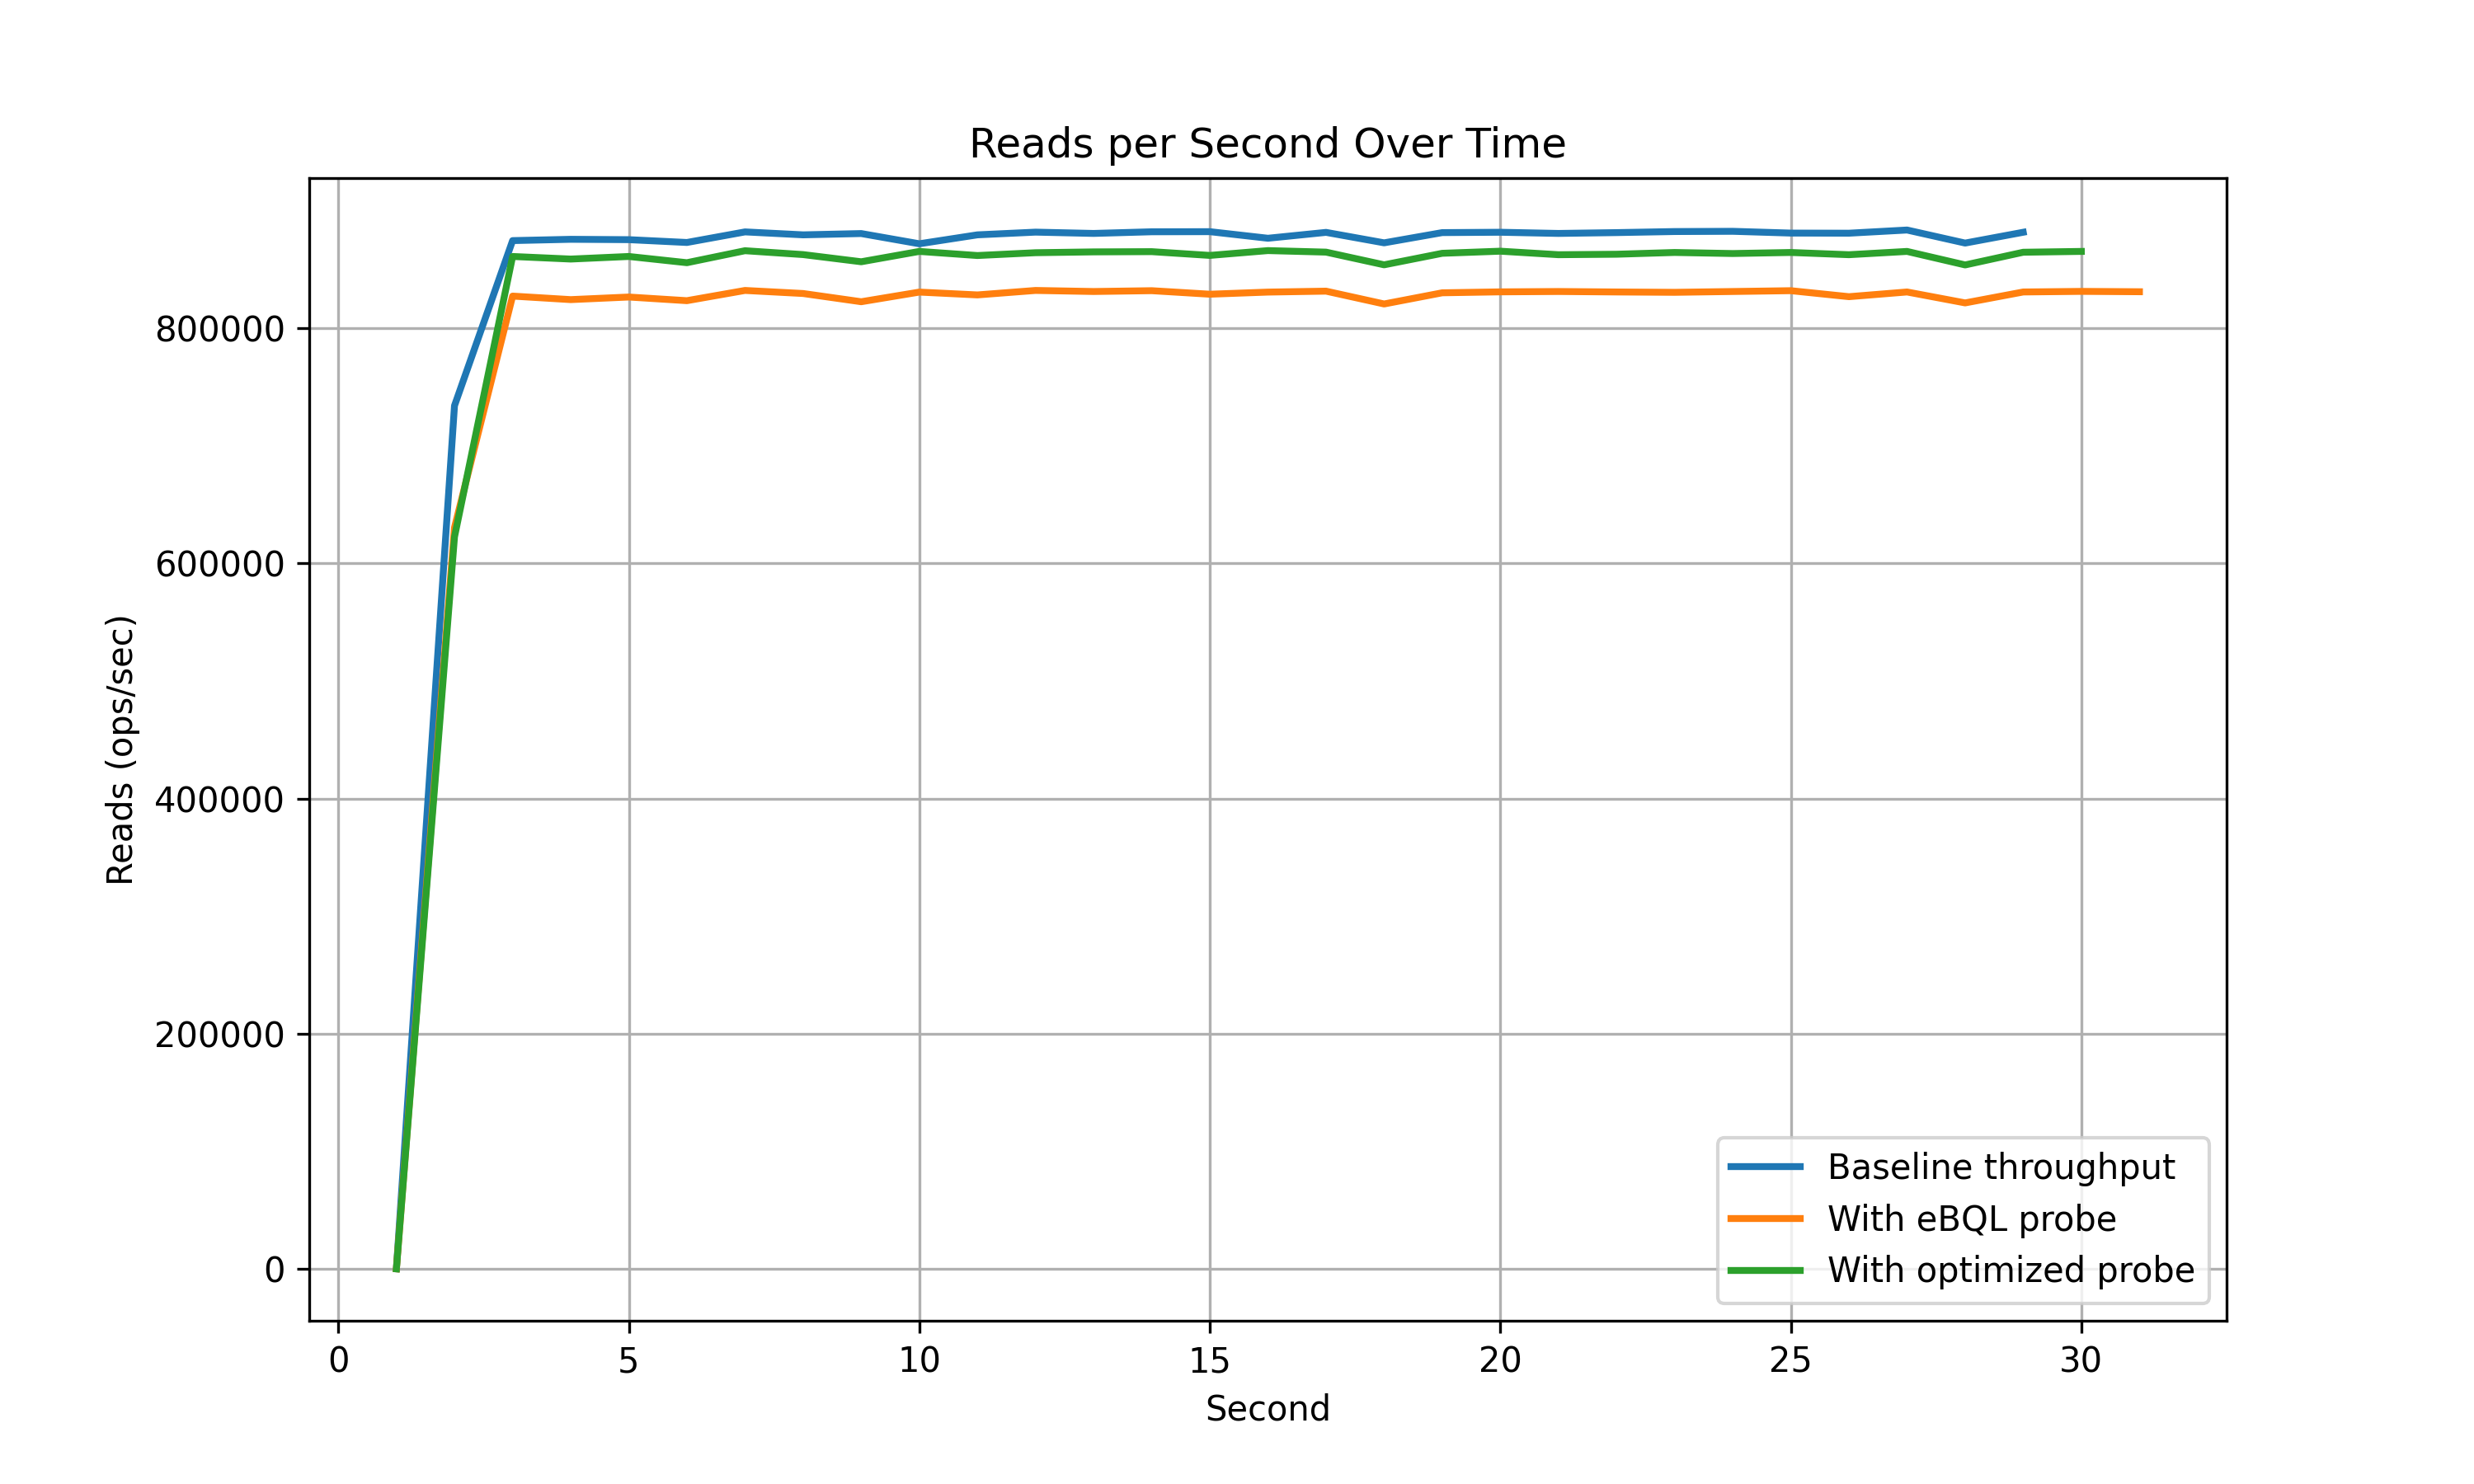
\includegraphics[width=0.6\textwidth]{diagrams/opt-eval-throughput.png}
    \caption{Throughput comparisons between baseline RocksDB without eBPF probes, with an
    eBQL-generated probe, and with a hand-optimized probe.}
    \label{fig:opt-eval-throughput}
\end{figure}

Using 8 worker threads across 12 CPUs, RocksDB achieves a baseline read throughput of $\sim 852k$
operations/second without any probes attached. Once the eBPF probe is attached, the read throughput
drops to $\sim 825k$ operations/second. Using the optimized probe, the read throughput is maintained
at $\sim 838k$ operations/second. Equivalently, the eBQL-generated probe incurs a $3.2\%$ overhead
on reads, compared to the hand-optimized probe's $1.7\%$ overhead.

\begin{figure}[htpb]
    \centering
    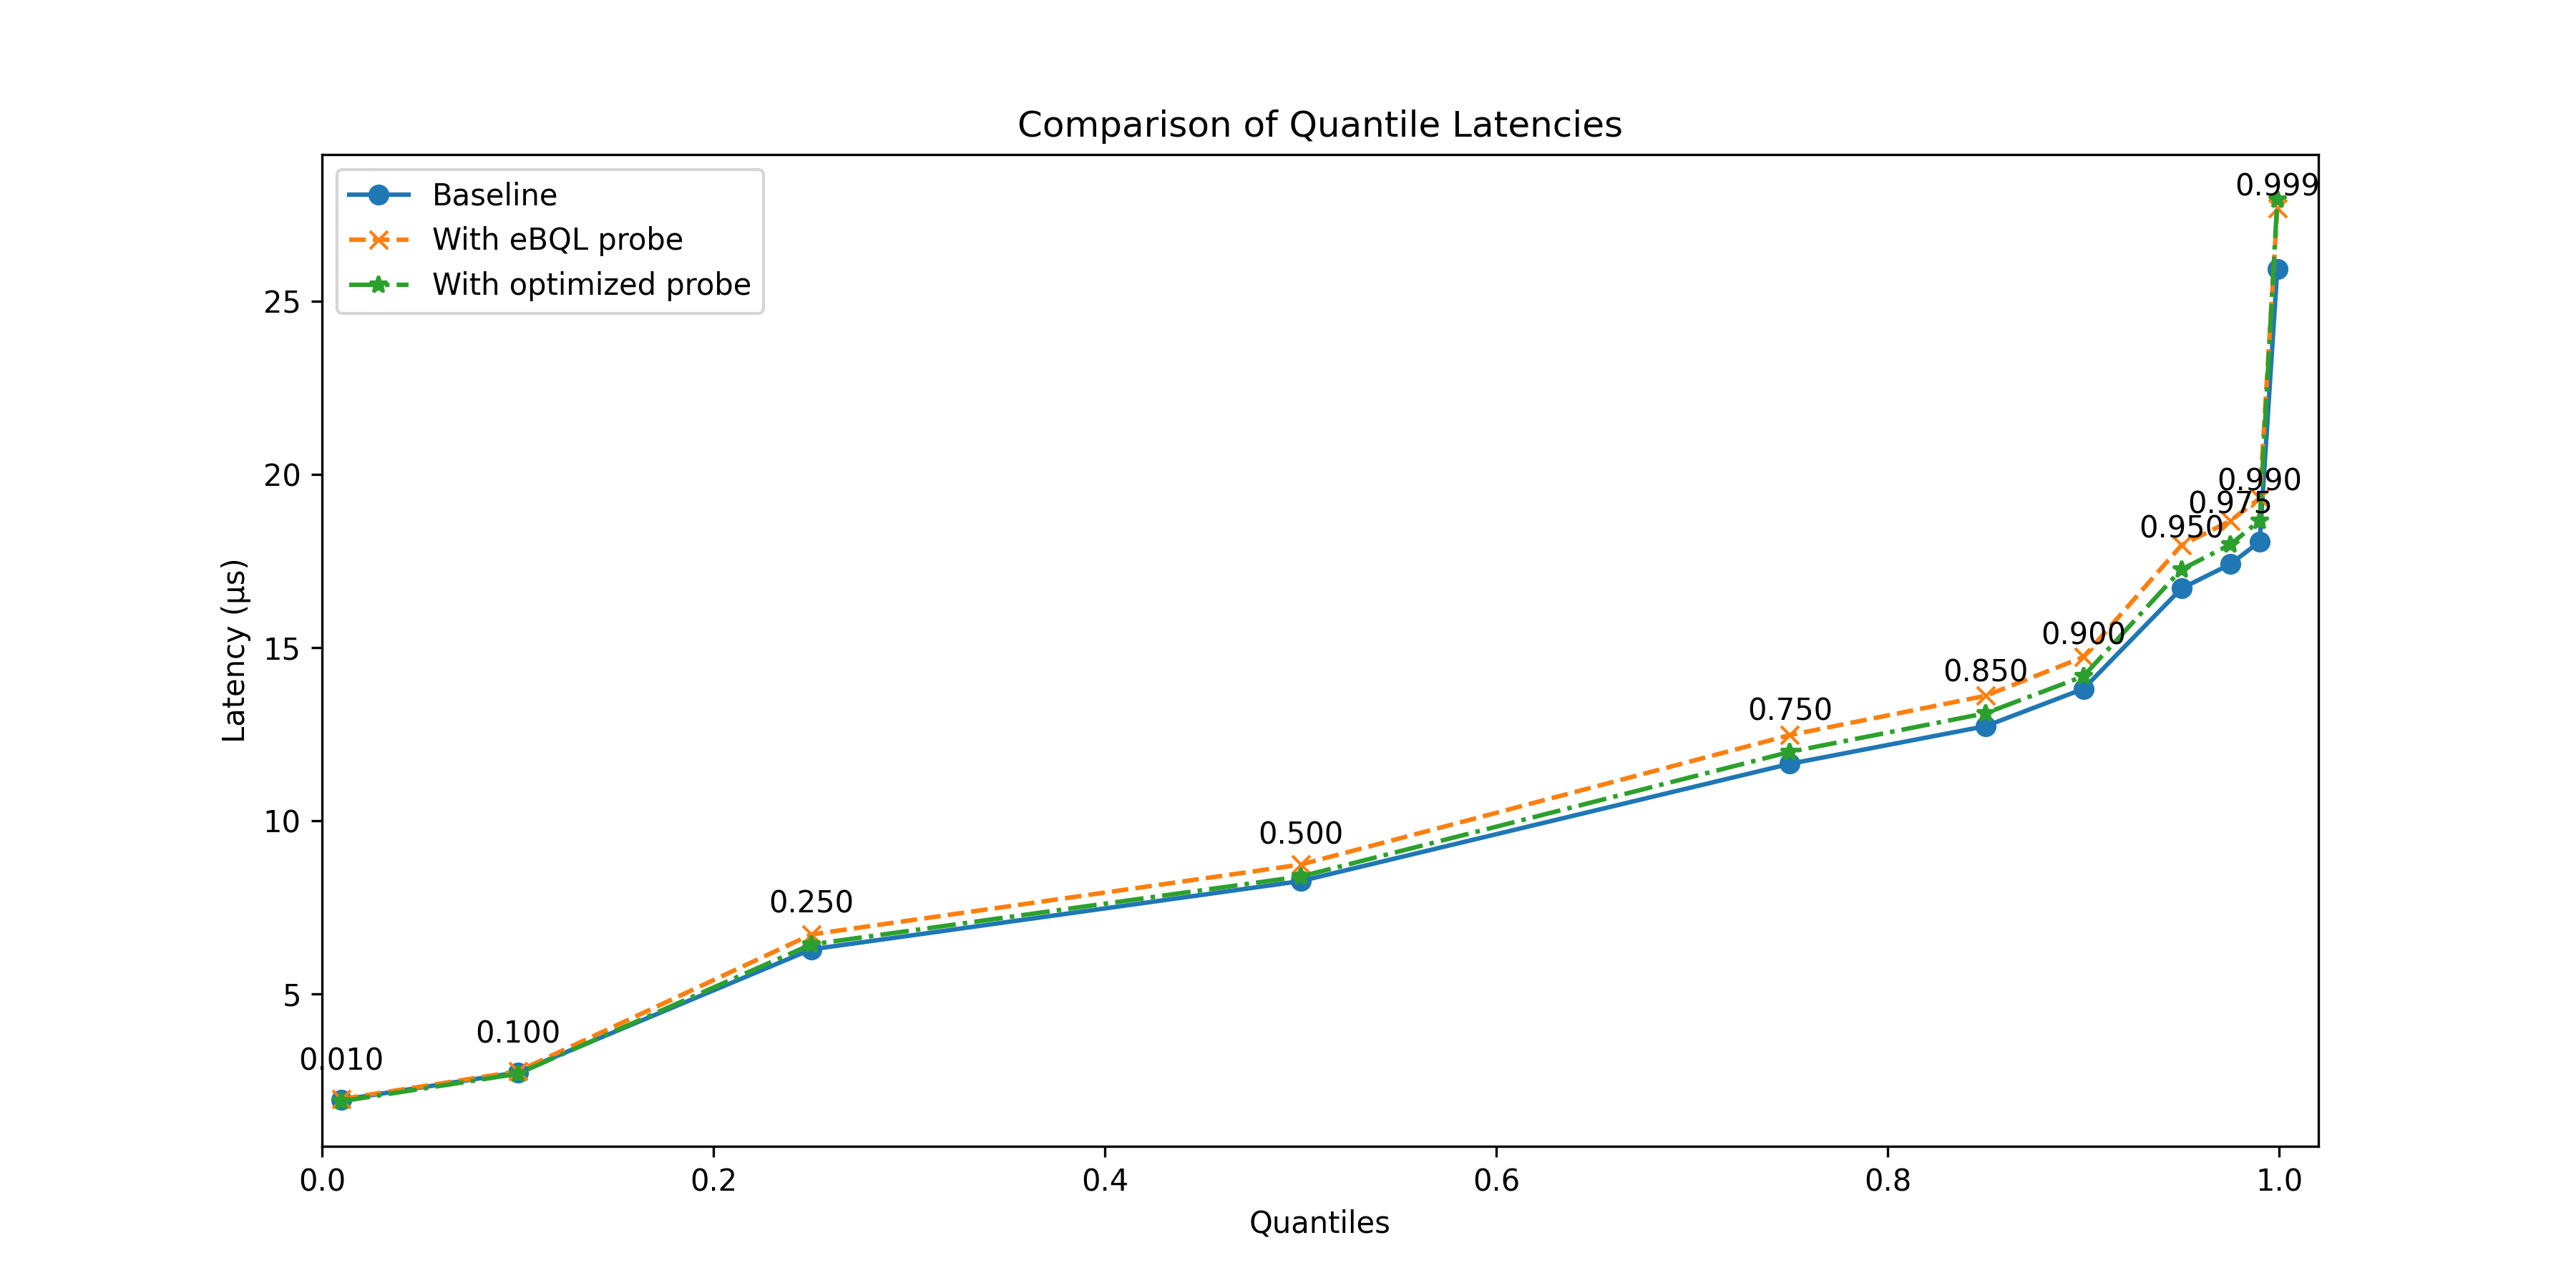
\includegraphics[width=0.8\textwidth]{diagrams/opt-eval-quantiles.png}
    \caption{Quantile comparisons between baseline RocksDB without eBPF probes, with an
    eBQL-generated probe, and with a hand-optimized probe.}
    \label{fig:opt-eval-quantiles}
\end{figure}

A similar result is seen in the quantile measurements: on average ($50\%$ quantile), the baseline
RocksDB read latency without an eBPF probe is $8.338\mu$s, versus $8.606\mu$s with the eBQL probe
($3.2\%$ overhead) and $8.456\mu$s ($1.4\%$ overhead). Despite deferring aggregation computations
and emitting to user-space until the window tumbles, the tail latency is not drastically affected
with the eBPF probe: at the tail ($99.9\%$ quantile) the baseline RocksDB read latency is
$22.437\mu$s, compared to $23.329\mu$s with the eBQL probe ($4.0\%$ overhead) and $22.969\mu$s with
the hand-optimized probe ($2.3\%$ overhead).

\subsection{Evaluation with Baseline eBPF Programs}
\label{baseline-eval}

We then measure the performance compared to a standard baseline eBPF query implementation using
only basic eBPF functionality, one that would feasibly be implemented as a HFT data collection
program.

We use the program presented in Figure \ref{code:pread64-unopt} as the baseline. Although simple,
the pre-requisites to develop an eBPF program like this is non-trivial, requiring knowledge of
tracepoint format and available contexts, program types, BPF helper functions, BPF maps, and the
ringbuf API (ref: bpf-ringbuf nakryiko); moreover, developers must be aware of the verifier
requirements; omitting the null check (\texttt{!q}) outputs a confusing error message that would
require knowledge of eBPF bytecode to decipher.

Compared to the purely kernel-space processing in the eBQL-generated program, the baseline program
defers all query computation to user-space; specifically, since only the raw record is emitted, the
user-space side must handle max/count/average aggregations, groupings, and windowing. This
complicates performance benchmarking. Raw throughput is no longer a fully accurate indicator of
program overhead: instead of the query functionality directly impacting throughput (as eBPF programs
run in kernel context, on the same process, after a hook point is triggered), the vast majority of
query functionality is handled in a separate process managing the eBPF probe.

Thus, for this benchmark we instead measure total CPU cycles as a function of work executed across
both the RocksDB application and the process managing the eBPF probe. This way, the additional query
work is accounted for, even if it did not directly affect throughput. For a direct conversion, on
our machine 100 CPU cycles is 1 second; this value can be determined with
\texttt{sysconf(\_SC\_CLK\_TCK)}. For this, we use \texttt{/proc/<pid>/stat} from \texttt{procfs}
for process cycles, and the BPF subsystem itself for BPF program cycles (via
\texttt{/proc/sys/kernel/bpf\_stats\_enabled}).

We measure five categories of CPU cycles: RocksDB user mode cycles, RocksDB kernel mode cycles, BPF
probe cycles, BPF management process user cycles, and BPF management process kernel cycles. From
these, we can additionally compute the overhead of the BPF subsystem itself by subtracting the
baseline RocksDB kernel mode cycles (the kernel mode cycles for RocksDB-specific work, like
\texttt{pread64} syscalls) and the BPF probe cycles (the BPF probe processing cycles) from the
RocksDB kernel mode cycles with the eBQL/standard-probe attached. To limit variance, we run each
program $50$ times, then compute the average cycle count among all invocations.

\begin{figure}[htpb]
    \centering
    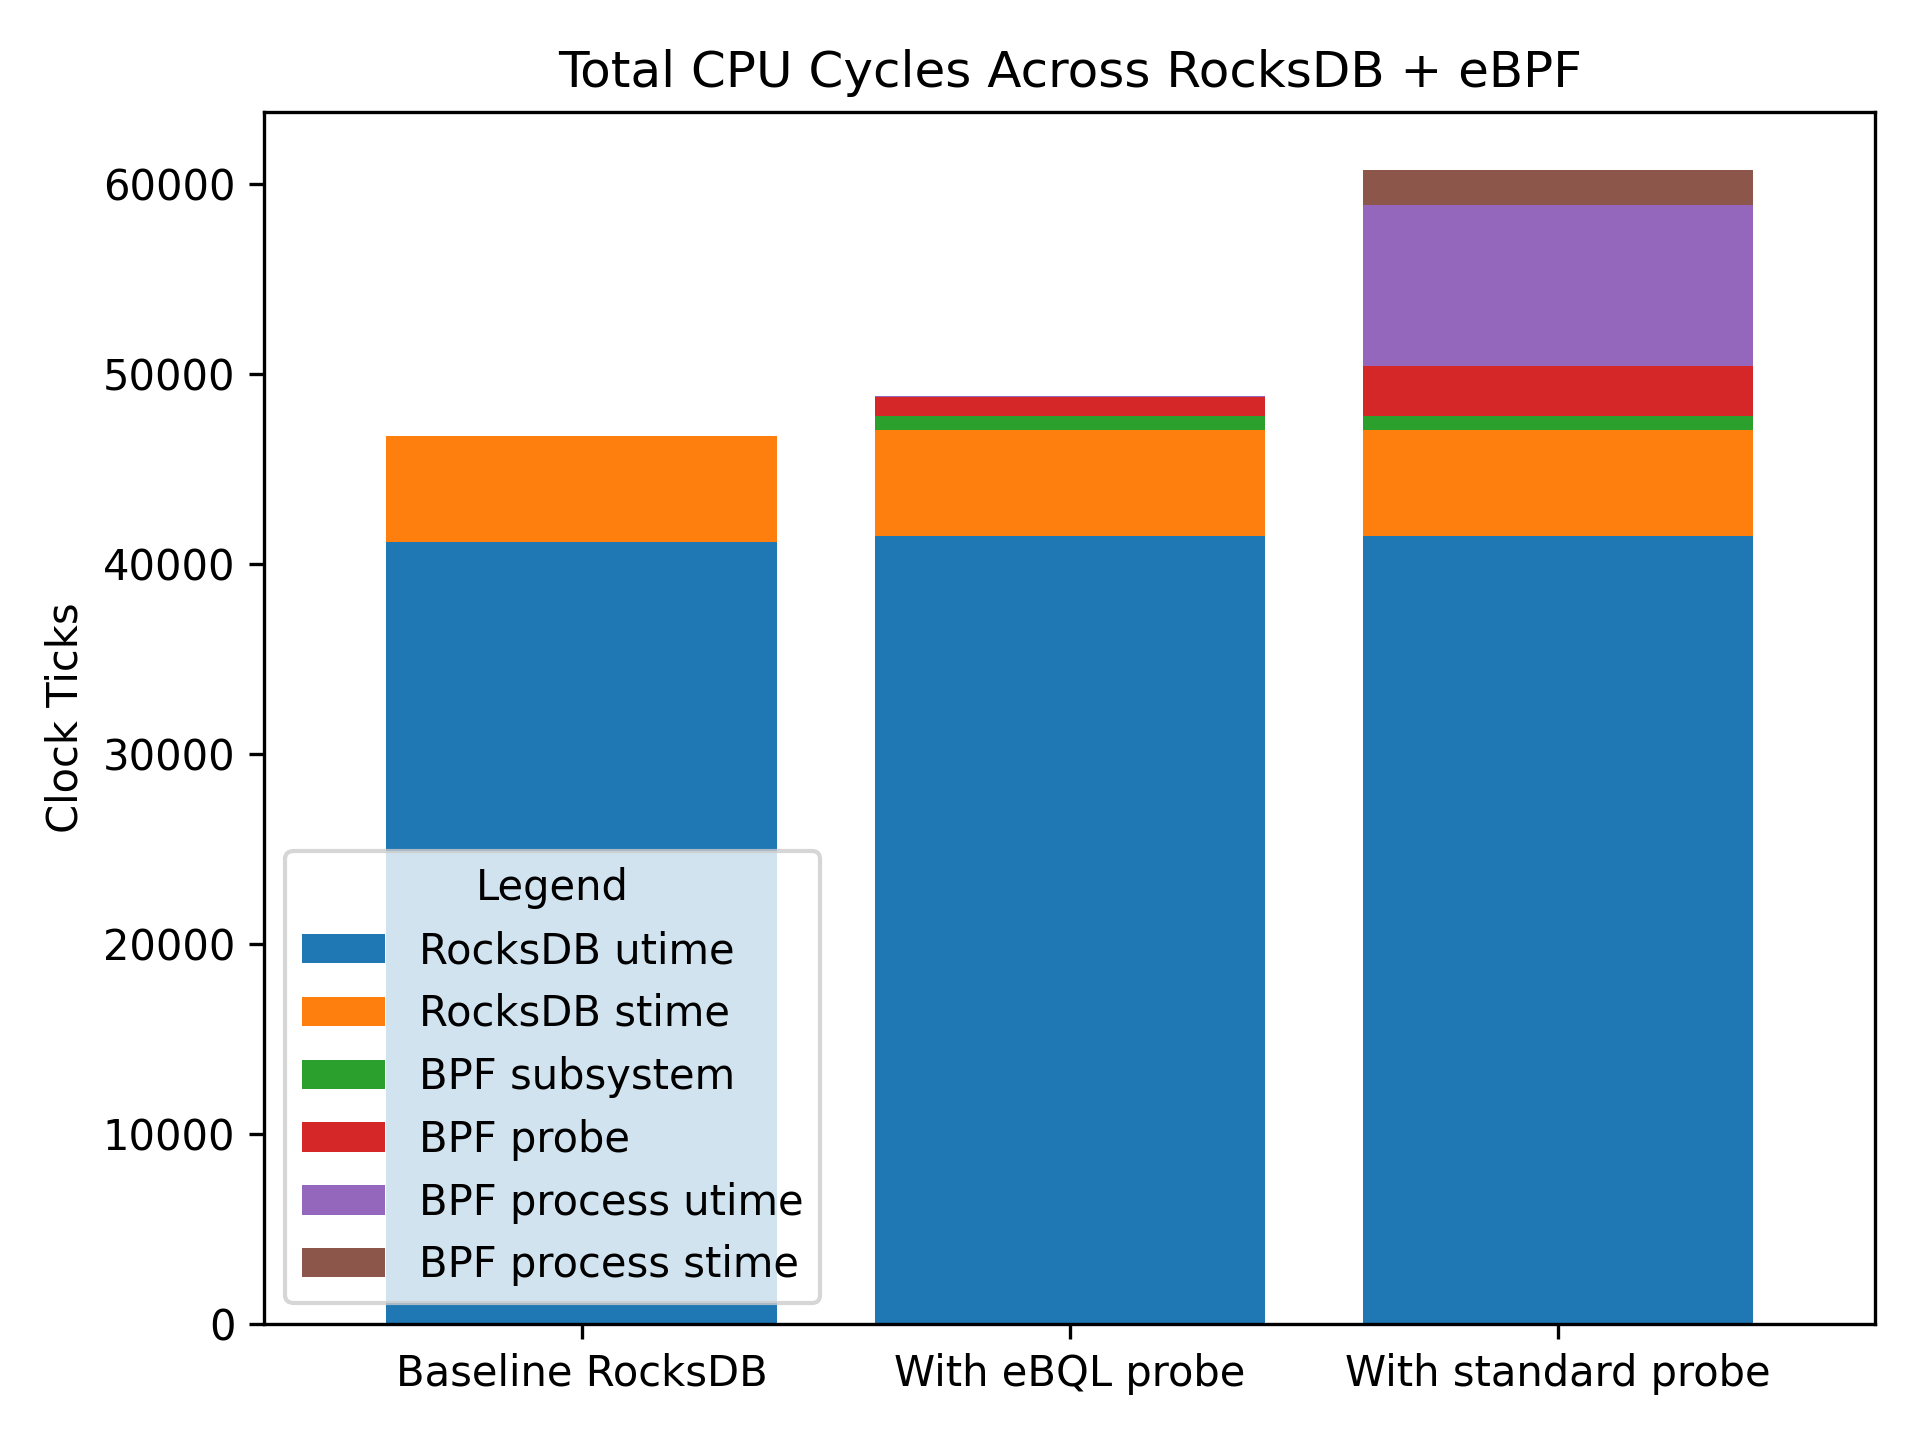
\includegraphics[width=0.6\textwidth]{diagrams/baseline-eval-cycles.png}
    \caption{CPU cycles used between RocksDB without eBPF probes, with an eBQL-generated probe, and
    with a standard probe.}
    \label{fig:baseline-eval-cycles}
\end{figure}

Figure \ref{fig:baseline-eval-cycles} shows the results, and Table \ref{tab:baseline-eval-nums}
contains detailed latency numbers (converted from CPU cycles). Across all programs, the utime/stime
for the RocksDB application itself remained roughly equivalent ($~41450$ cycles). Likewise, the
overhead from the BPF subsystem itself was relatively consistent across programs ($\sim 120$ns per
BPF probe invocation).

\begin{table}[htpb]
    \centering
    \caption{BPF program latencies per run}
    \label{tab:baseline-eval-nums}
    \begin{tabular}{| l | l | l | l |}
        \hline
        \multicolumn{1}{|c|}{\textit{\textbf{Program}}} &
        \multicolumn{1}{c|}{\textit{\textbf{Probe runtime (avg/run)}}} &
        \multicolumn{1}{c|}{\textit{\textbf{BPF subsystem overhead (avg/run)}}} &
        \multicolumn{1}{c|}{\textit{\textbf{Run count}}}
        \tabularnewline \hline
        eBQL & 10.0852s (167.031ns) & 7.587s (125.656ns) & 60379284 \\
        \hline
        Standard & 26.561s (439.708ns) & 7.105s (117.622ns) & 60406223 \\
        \hline
    \end{tabular}
\end{table}

Perhaps surprisingly, despite performing less computation in-kernel, the
standard BPF program actually incurs \textit{more} overhead per BPF probe execution (we investigate
this below, in \S \ref{perf-drilldown}). Further, the managing process must now also devote
significant CPU time towards computing the aggregations in user-space and polling for more data from
kernel-space.

As expected, the standard BPF program consumes more CPU cycles to perform the same query. To further
investigate, we evaluate each probe end-to-end, measuring RocksDB read throughput when both
processes are run on 12 CPUs as before, then on 8 CPUs to simulate a resource-constrained
environment.

Figure \ref{fig:baseline-eval-throughput} shows the results. From the CPU cycles evaluation before,
the 12 CPUs end-to-end evaluation is expected: the eBQL probe outperforms the standard eBPF probe
with less overhead ($3.2\%$ vs $7.2\%$). Further, when constrained to 8 CPUs (and thus the RocksDB
process and the process performing user-space query processing are competing for CPU cycles), the
standard eBPF probe's performance further deteriorates ($17.6\%$ overhead) while the eBQL probe's
performance remains the same.

\begin{figure}
    \centering
    \begin{subfigure}{.5\textwidth}
        \centering
        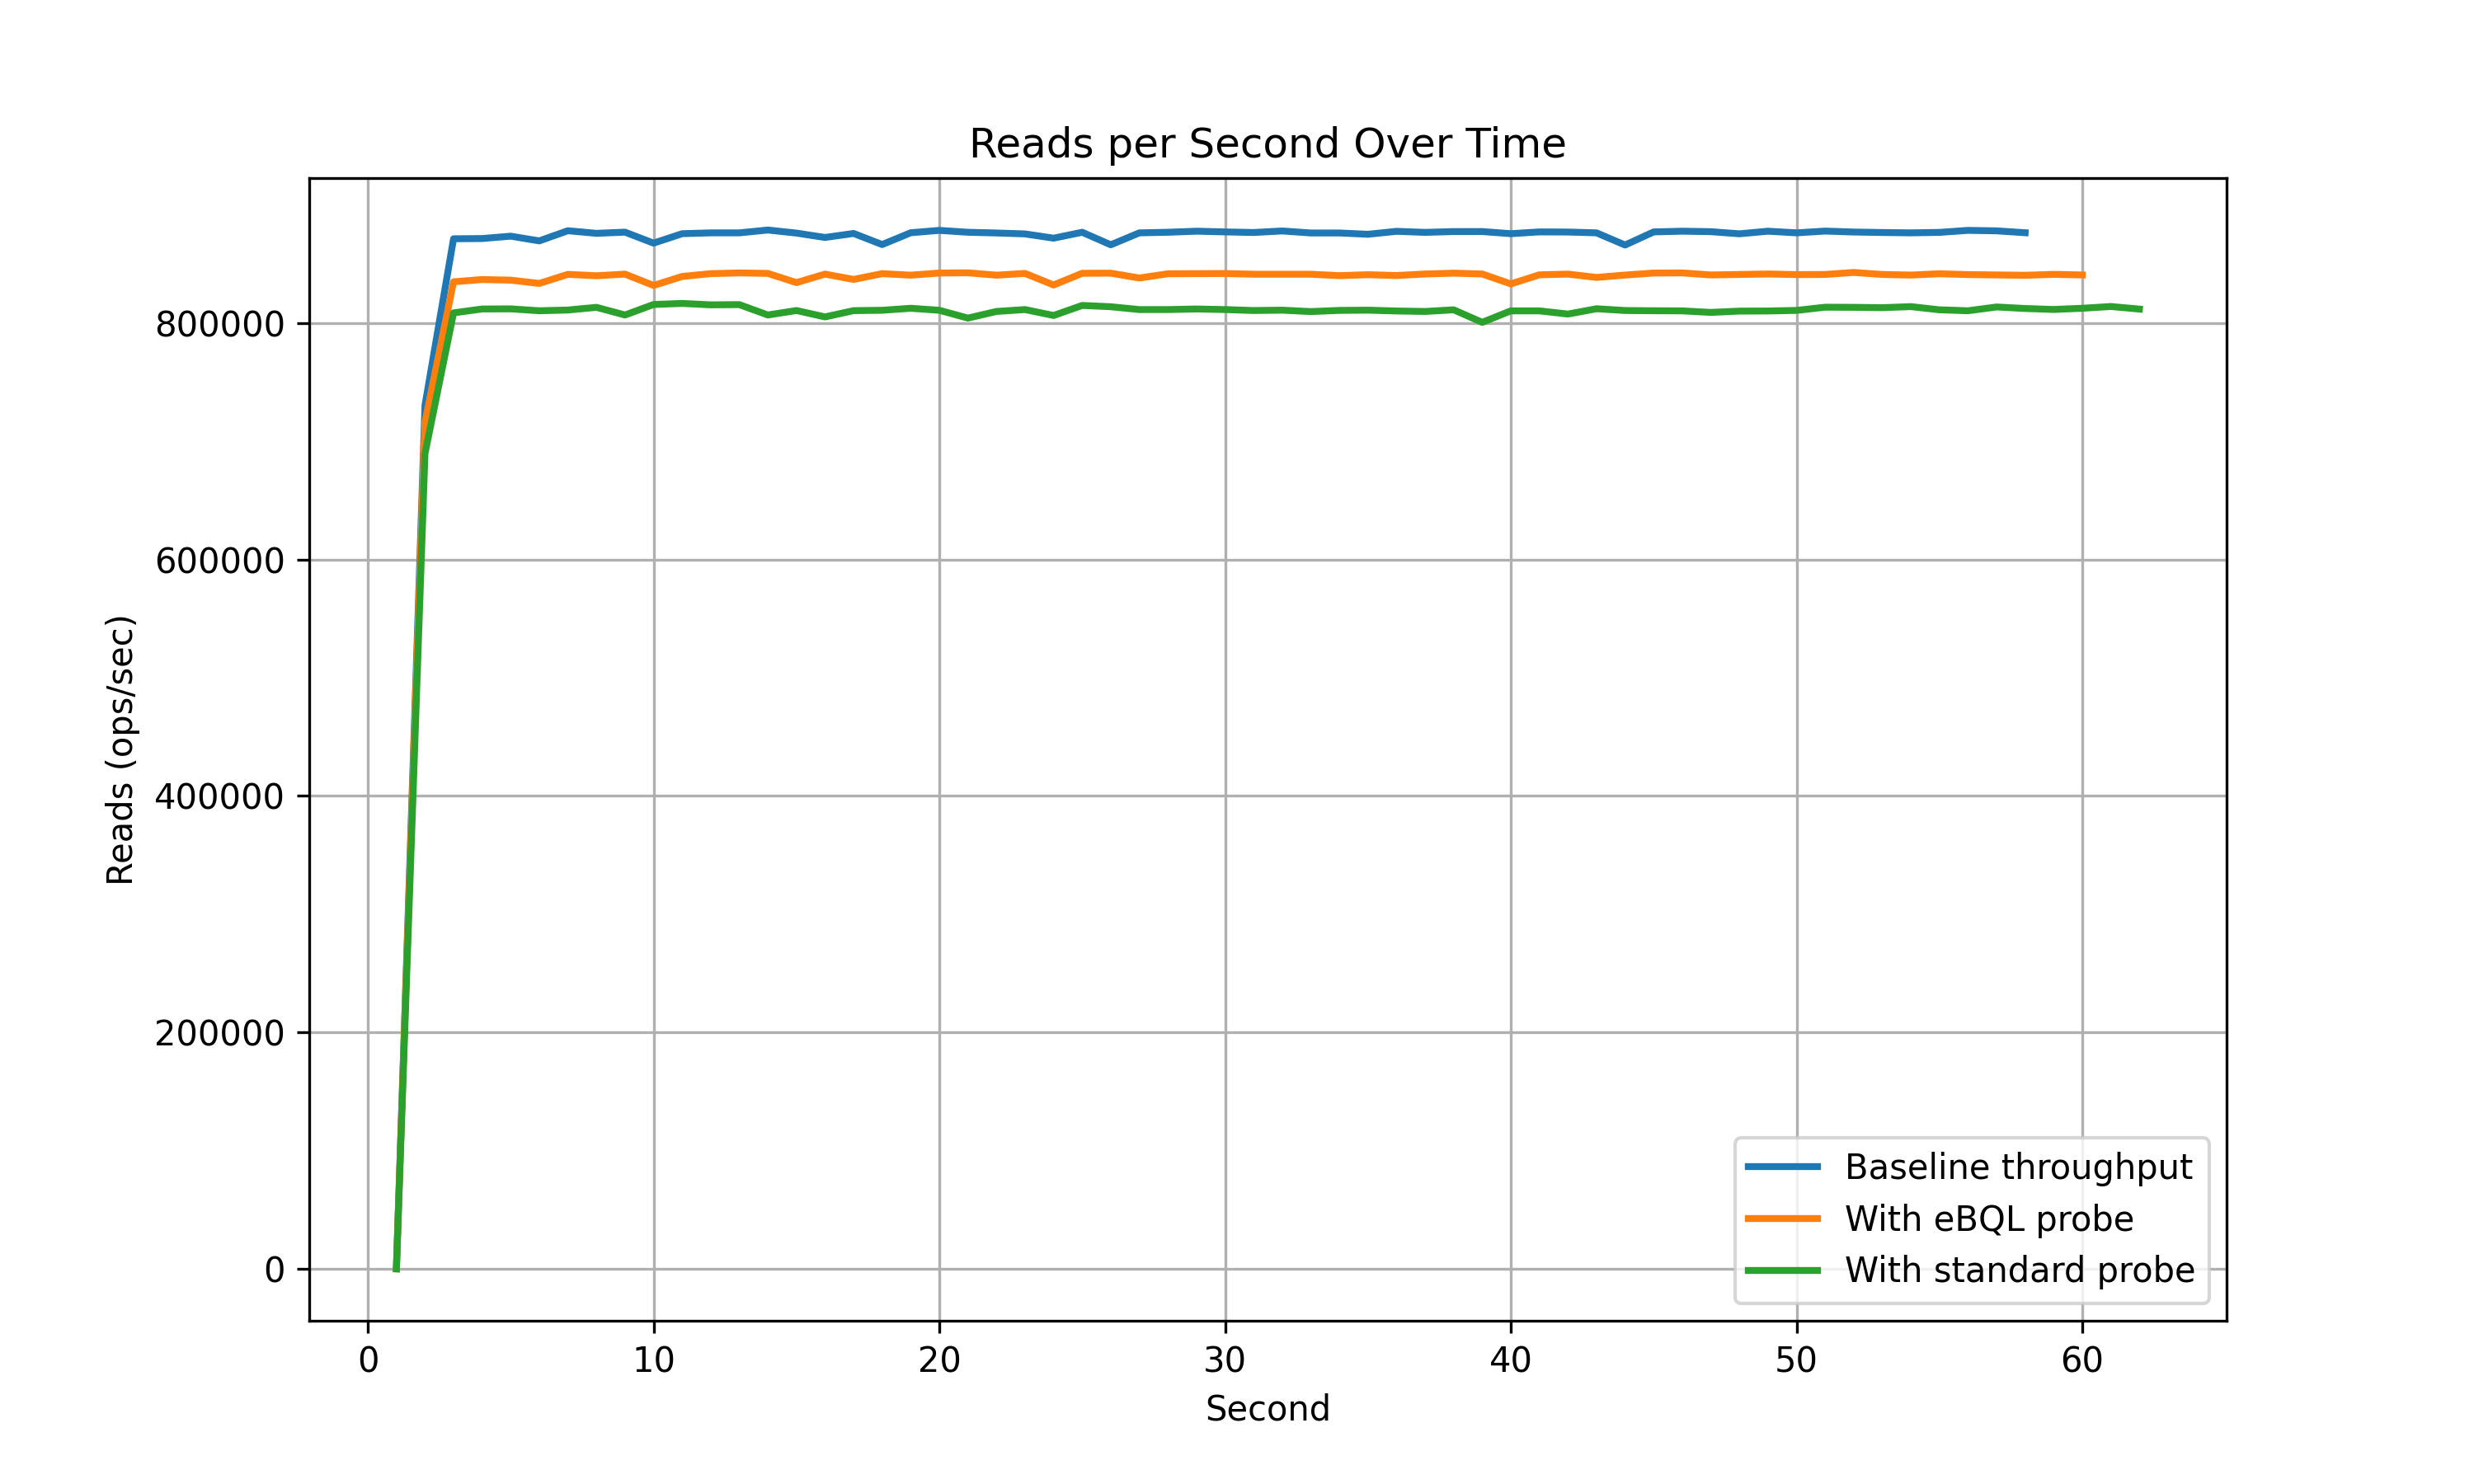
\includegraphics[width=\linewidth]{diagrams/baseline-eval-throughput-12.png}
        \caption{}
        \label{fig:sub1}
    \end{subfigure}%
    \begin{subfigure}{.5\textwidth}
        \centering
        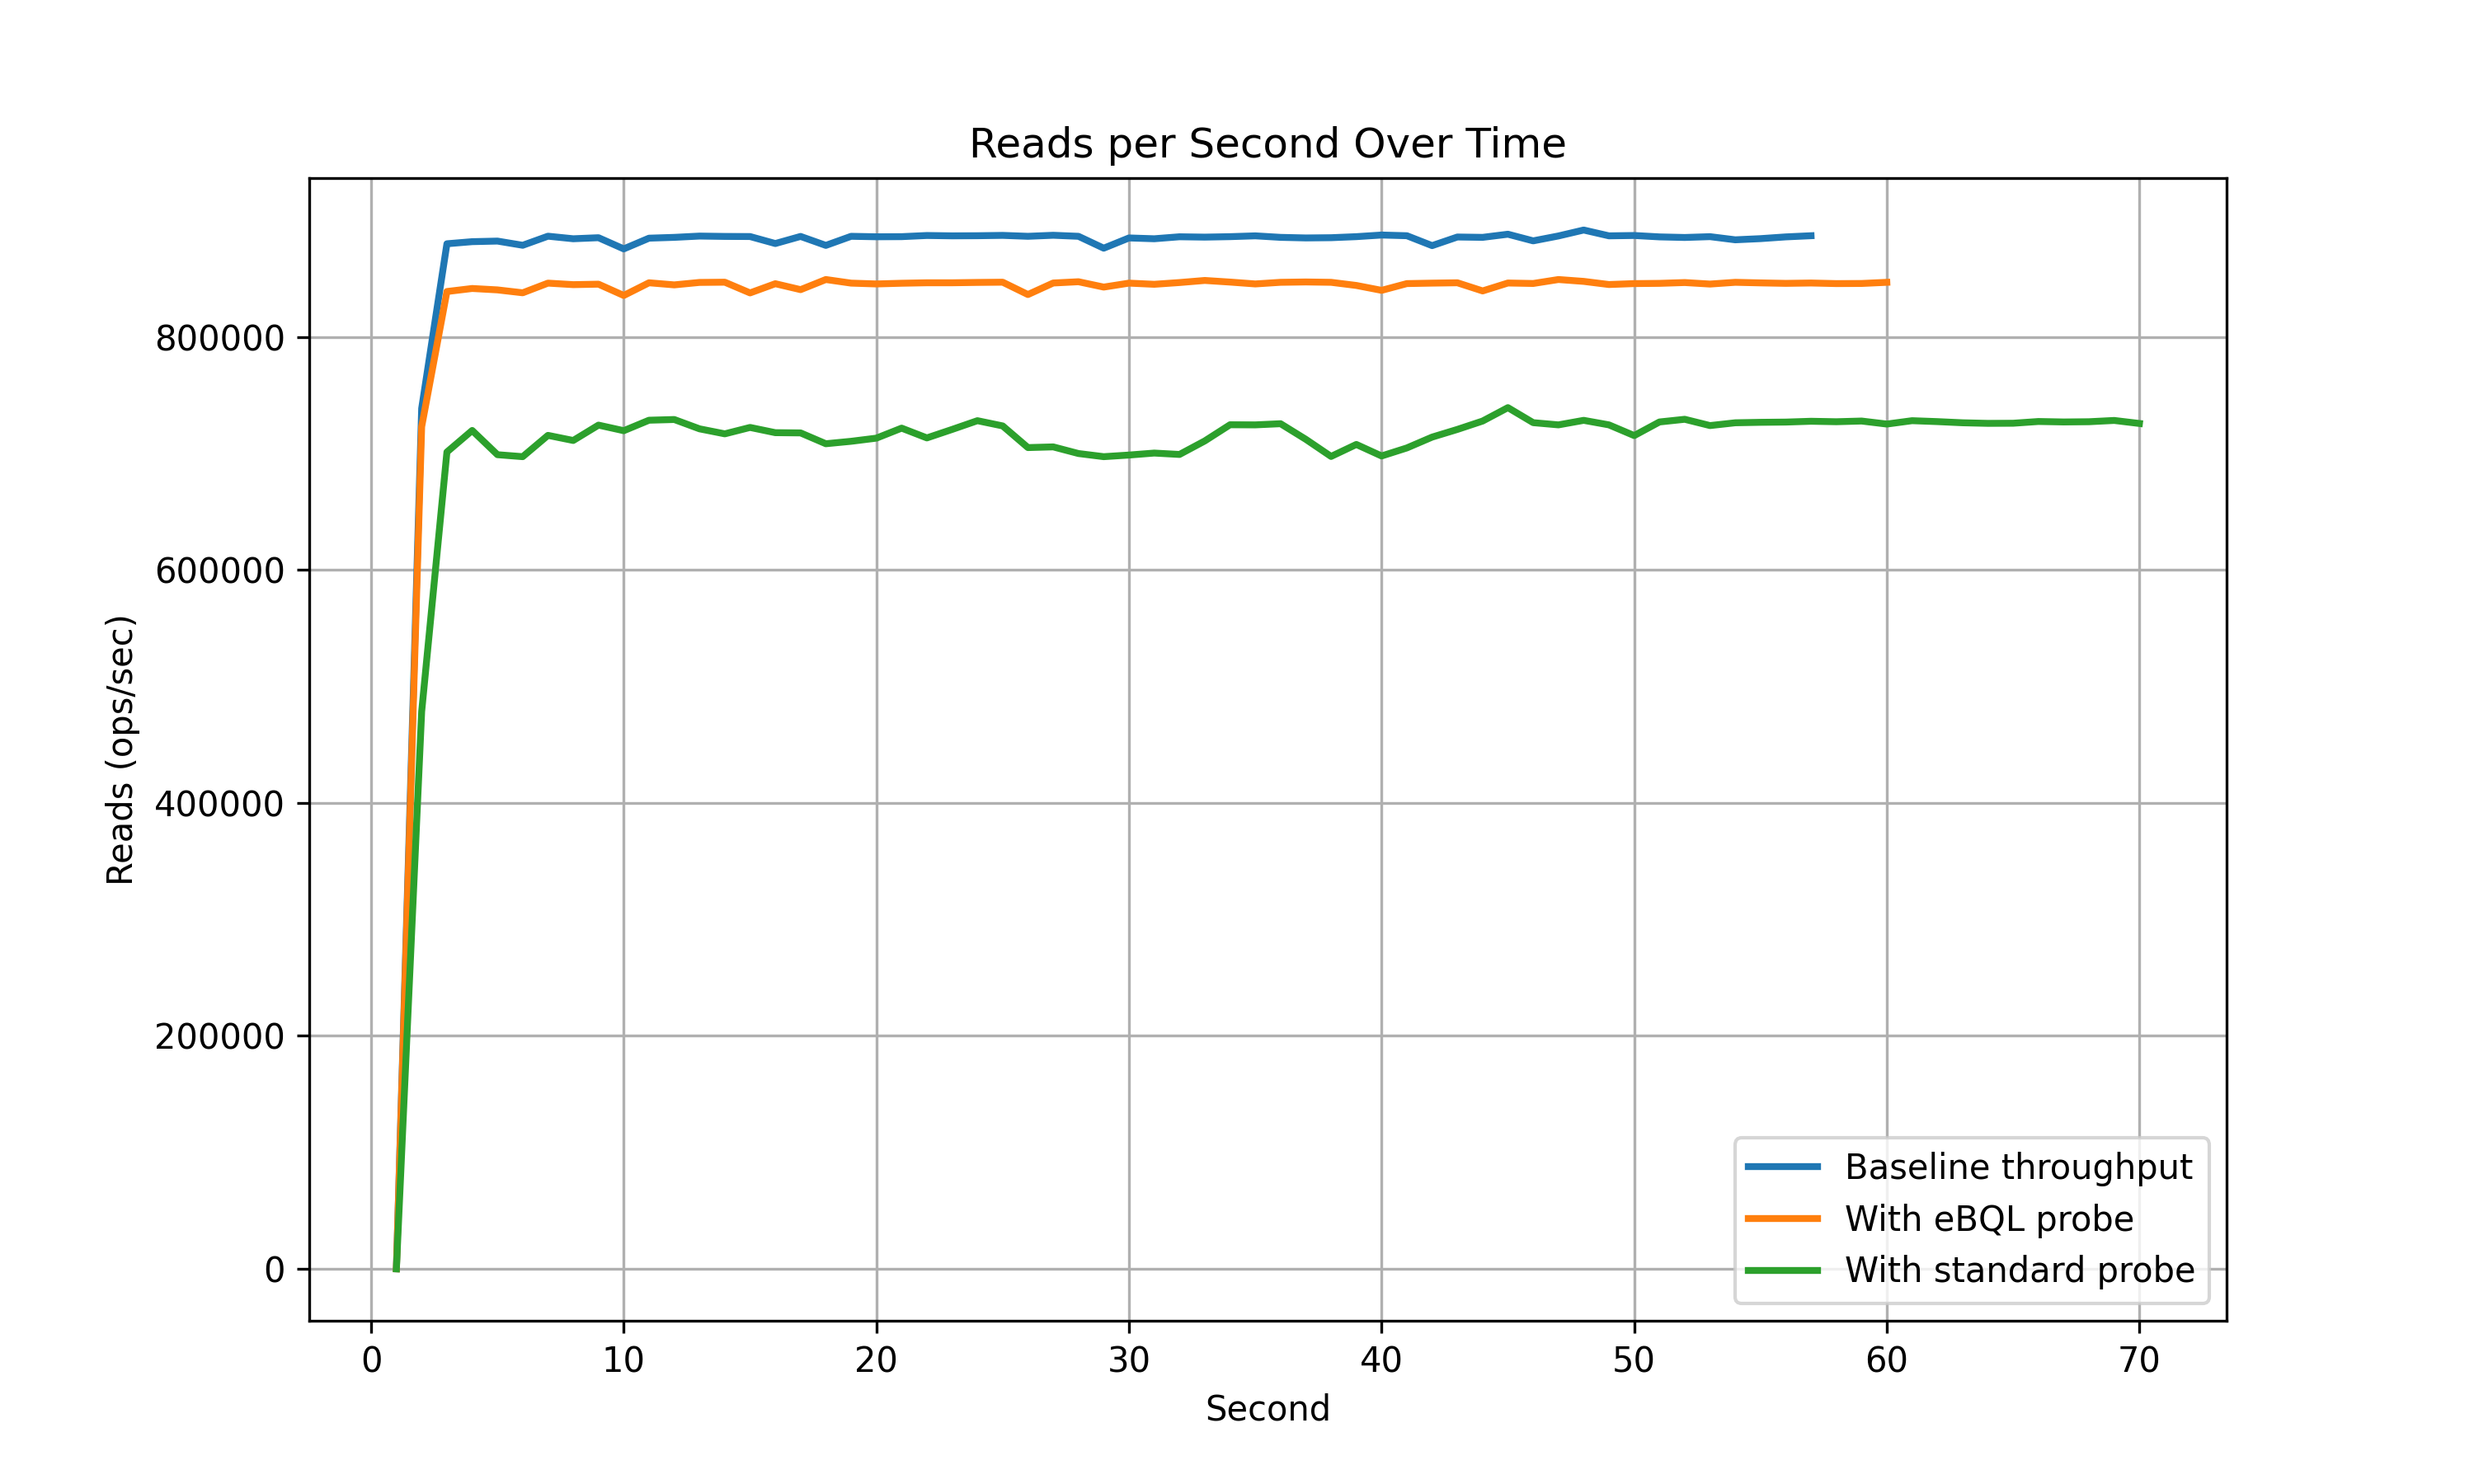
\includegraphics[width=\linewidth]{diagrams/baseline-eval-throughput-8.png}
        \caption{}
    \end{subfigure}
    \caption{End-to-end read throughput comparison on 12 (a) and 8 (b) CPUs.}
    \label{fig:baseline-eval-throughput}
\end{figure}

\subsection{Performance Drilldown}
\label{perf-drilldown}

We briefly investigate the cause behind standard probe's high overhead.

\begin{figure}
    \centering
    \begin{subfigure}{.8\textwidth}
        \centering
        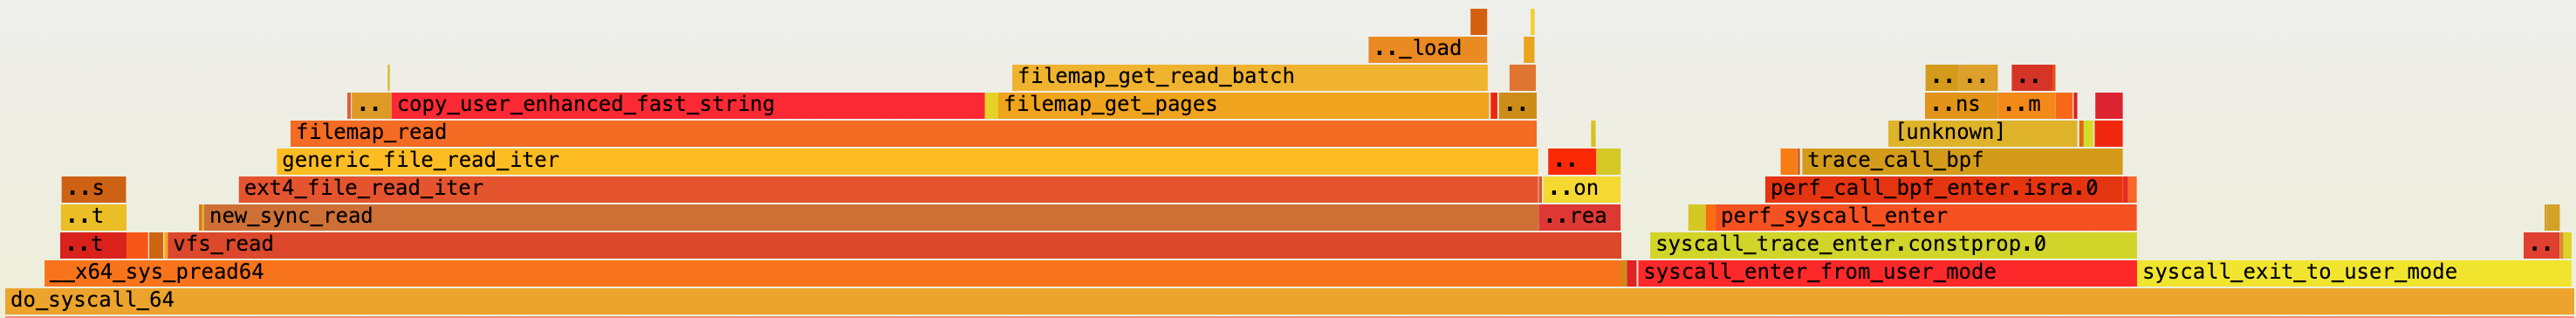
\includegraphics[width=\linewidth]{diagrams/opt-pread-fg.png}
        \caption{}
    \end{subfigure}

    \begin{subfigure}{.8\textwidth}
        \centering
        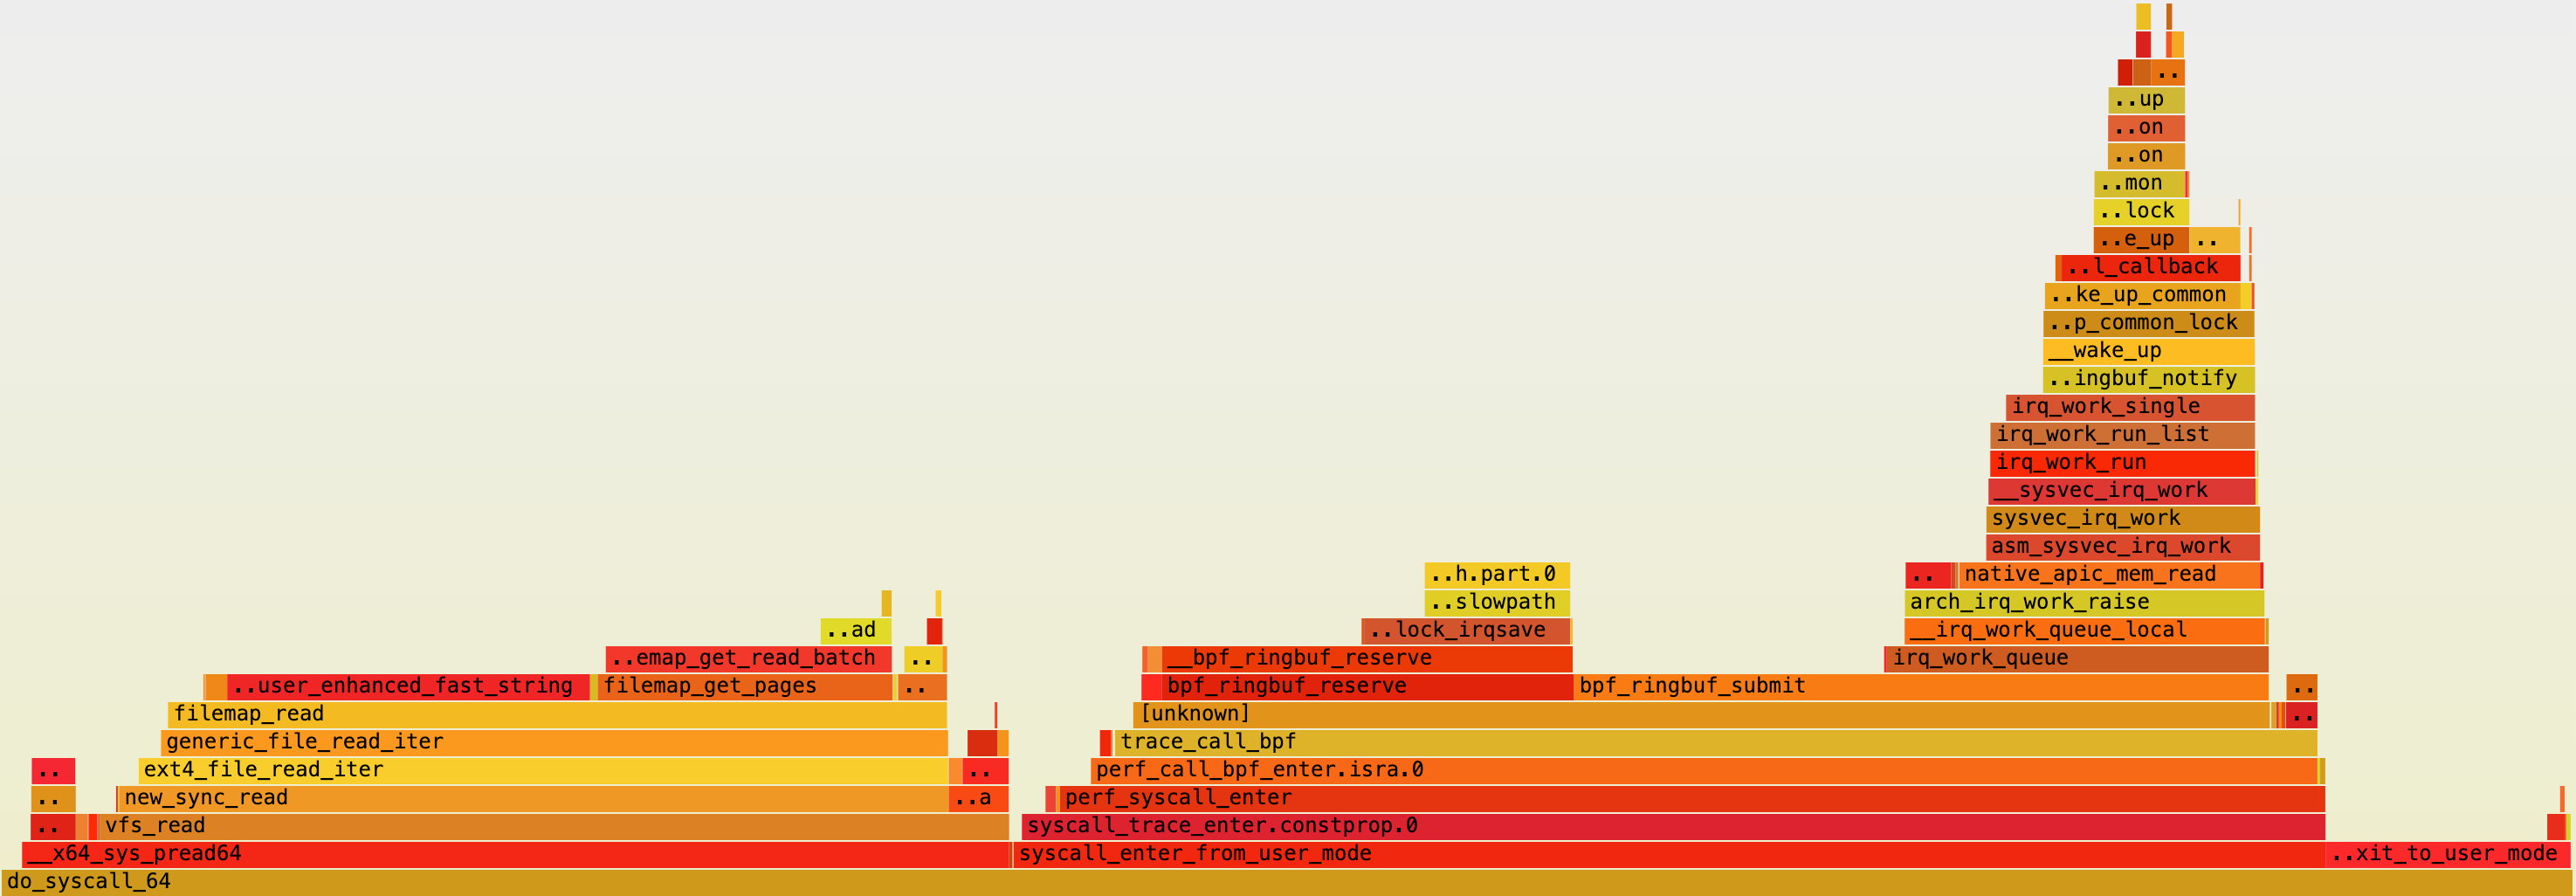
\includegraphics[width=\linewidth]{diagrams/unopt-pread-fg.png}
        \caption{}
    \end{subfigure}
    \caption{Flamegraphs of RocksDB's \texttt{pread64} syscall under the eBQL probe (a) and standard
    probe (b).}
    \label{fig:pread-fgs}
\end{figure}

Figure \ref{fig:pread-fgs} shows two flamegraphs comparing RocksDB's \texttt{do\_syscall\_64} stack
trace and rough execution proportions under an eBQL probe, and the standard probe. In the standard
probe, more than half the \texttt{pread64} syscall's time is spent in the BPF probe itself, in
particular reserving and submitting values to the BPF ring buffer to transmit values to user-space;
in contrast, only a small fraction of time is spent within the eBQL probe, with the two highest
overhead functions being hash map lookups and retrieving the \texttt{ktime}.

This also shows the BPF subsystem's overhead: in both programs, both entering the BPF program from
the syscall context and exiting the BPF program into user mode incur a non-trivial penalty (which
can be quantified from Table \ref{tab:baseline-eval-nums}).

\subsection{Discussion}

eBQL's probe itself, despite performing aggregations every time the window tumbles, manages to
maintain a low tail latency. On average, the probe runs for $\sim 160$ns, with around $\sim 120$ns
spent on infrastructure supporting the hook.

While eBQL is not a complete zero-cost abstraction, it only incurs minimal additional overhead over
the hand-optimized eBPF program, and provides significant performance improvements over a standard
eBPF probe that are only exacerbated in a resource-constrained environment. Further, in most cases,
the performance gap between eBQL and hand-optimized code is closeable. For instance, the key
optimization between eBQL and the hand-optimized code is utilizing per-CPU maps, since one of the
group-by keys was CPU. If eBQL's query optimizer can identify special cases to use per-CPU or
task-local storage, it is likely that eBQL probes can become on-par with hand-optimized code, with a
fraction of the development effort.
